\documentclass{atistandalonetask}
\usepackage{atistandard}

\begin{document}
  \begin{atiTask}[
    title = Integrale mit Delta-Distributionen I
  ]
	Berechnen Sie die Integrale:

    \begin{atiSubequations}
    	\begin{multicols}{2}
    	\item{\integral{-3}{0}{\delta(x-1)}{x}}
    	\item{\integral{-1}{1}{e^x\delta(x)}{x}}
    	\item{\integral{-\infty}{\infty}{\cos x\delta(x-\pi)}{x}}
    	\item{\integral{-\infty}{3}{\cos x\delta(x-\pi)}{x}}
    	\item{\integral{-\infty}{\infty}{xf(x)\delta(x}{x}}
    	\item{\integral{-\infty}{\infty}{(x^2+3)\delta(5-x)}{x}}
   \end{multicols}	
  
   \end{atiSubequations}
    \atiNote{Gibt es Einschränkungen an $f(x)$ in (v)?}
  \end{atiTask}
  \begin{atiSolution}
   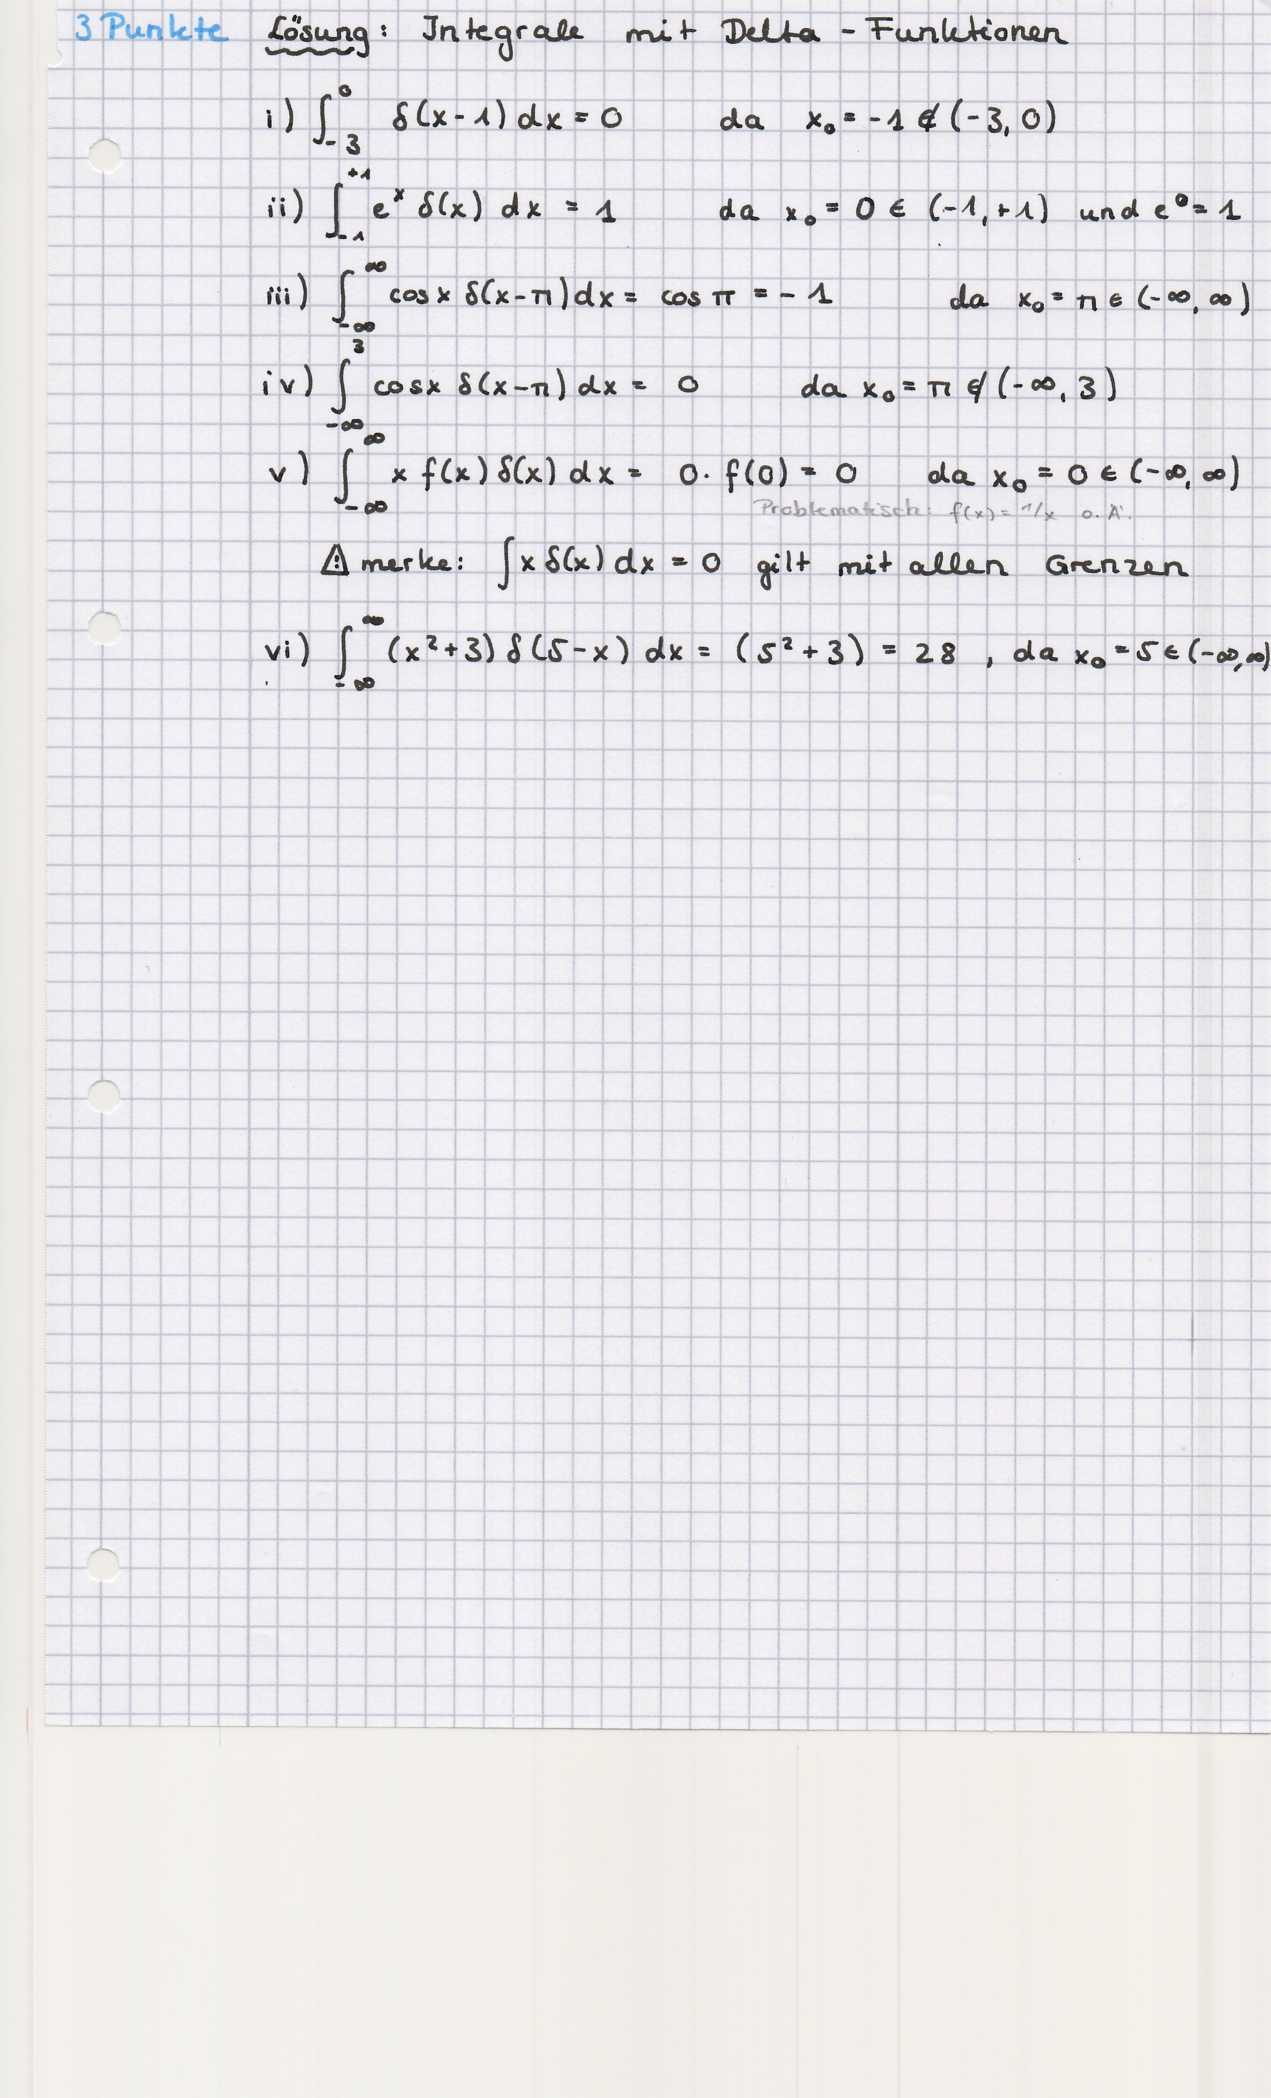
\includepdf[pages=-]{solution-delta_ii.pdf}
  \end{atiSolution}
\end{document}